\textit{This section was contributed by William Durkin}.

This cookbook is a modification of the previous example that explores changes in the way topography develops when a 
highly viscous crust is added.  
In this cookbook, we use a material model in which the material changes from low
viscosity mantle to high viscosity crust at $z = z_j = \texttt{jump height}$,
i.e., the piecewise viscosity function is defined as
\begin{align*}
  \eta(z) = \left\{
    \begin{matrix}
      \eta_U & \text{for}\ z > z_j, \\
      \eta_L & \text{for}\ z  \le z_j.
    \end{matrix}
  \right.
\end{align*}
where $\eta_U$ and $\eta_L$ are the viscosities of the upper and lower layers,
respectively. This viscosity model can be implemented by creating a plugin that
is a small modification of the \texttt{simpler} material model (from which it
is otherwise simply copied). We call this material model ``SimplerWithCrust''.
In particular, what is necessary is an evaluation function that looks like this:
\begin{lstlisting}[frame=single,language=C++] 
    template <int dim>
    void
    SimplerWithCrust<dim>::
    evaluate(const typename Interface<dim>::MaterialModelInputs &in, 
             typename Interface<dim>::MaterialModelOutputs &out ) const
    {
      for (unsigned int i=0; i<in.n_evaluation_points(); ++i)
        {
          const double z = in.position[i][1];

          if (z>jump_height)
            out.viscosities[i] = eta_U;
          else
            out.viscosities[i] = eta_L;

          out.densities[i] = reference_density * (1.0 - thermal_expansion_coefficient * (in.temperature[i] - reference_temperature));
          out.thermal_expansion_coefficients[i] = thermal_expansion_coefficient;
          out.specific_heat[i] = reference_specific_heat;
          out.thermal_conductivities[i] = thermal_conductivity;
          out.compressibilities[i] = 0.0;
          out.entropy_derivative_pressure[i] = 0.0;
          out.entropy_derivative_temperature[i] = 0.0;
          for (unsigned int c=0; c<in.composition[i].size(); ++c)
            out.reaction_terms[i][c] = 0.0;
        }
    }
\end{lstlisting}

Additional changes make the new parameters \texttt{Jump height}, \texttt{Lower
viscosity}, and \texttt{Upper viscosity} available to the input parameter file,
and corresponding variables available in the class and used in the code snippet
above. The entire code can be found in
\url{cookbooks/free_surface_with_crust/plugin/simpler_with_crust.cc}. Refer to
Section~\ref{sec:plugins} for more information about writing and running
plugins.

The following changes are necessary compared to the input file from the
cookbook shown in Section~\ref{sec:cookbooks-freesurface} to include a crust:
\begin{itemize}
  \item Load the plugin implementing the new material model:
  \lstinputlisting[language=prmfile]{cookbooks/free_surface_with_crust/doc/free_surface_with_crust.part1.prm.out}
  
  \item Declare values for the new parameters:
  \lstinputlisting[language=prmfile]{cookbooks/free_surface_with_crust/doc/free_surface_with_crust.part2.prm.out}
  Note that the height of the interface at 170km is interpreted in the
  coordinate system in which the box geometry of this cookbook lives. The box
  has dimensions $500\si{km}\times 200\si{km}$, so an interface height of
  170km implies a depth of 30km.
\end{itemize}

The entire parameter file is located in
\url{cookbooks/free_surface_with_crust/free_surface_with_crust.prm}.

Running this input file generates a
crust that is 30 km thick and 1000 times as viscous as the lower layer.
Figure~\ref{fig:freesurfaceWC} shows that adding a crust to the model causes the maximum topography to both decrease and occur at a later time.
Heat flows through the system primarily by advection until the temperature anomaly reaches the base of the
crustal layer (approximately at the time for which Fig~\ref{fig:freesurfaceWC}
shows the temperature profile).
The crust's high viscosity reduces the temperature anomaly's velocity
substantially, causing it to affect the surface topography at a later time. Just
as the cookbook shown in Section~\ref{sec:cookbooks-freesurface}, the
topography returns to zero after some time.

\begin{figure}
  \centering
  
\includegraphics[height=0.25\textwidth]{cookbooks/free_surface_with_crust/doc/free_surface_with_crust.png}
  \hfill
  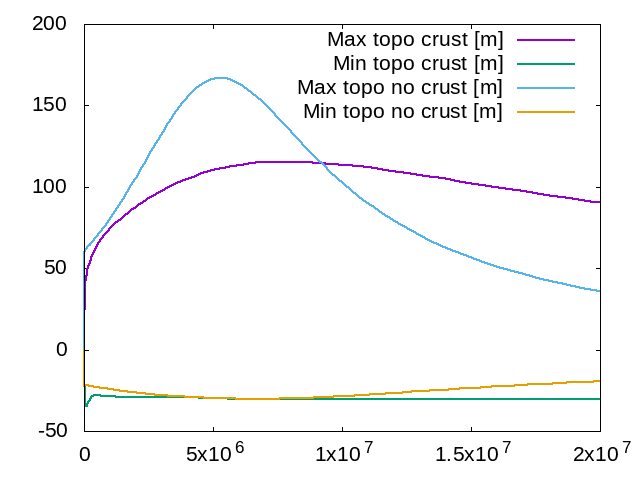
\includegraphics[height=0.25\textwidth]{cookbooks/free_surface_with_crust/doc/topography.png}
  \caption{\it Adding a viscous crust to a model with surface topography. The
  thermal anomaly spreads horizontally as it collides with the highly viscous crust (left, white solid line). The addition of a crustal layer both dampens and delays the appearance of the topographic maximum and minimum (right).}
  \label{fig:freesurfaceWC}
\end{figure}